\documentclass[11pt, spanish, a4paper]{article}
\usepackage[spanish]{babel}
\usepackage[top=0.5in]{geometry}
\selectlanguage{spanish}
\usepackage[utf8]{inputenc}
\usepackage{hyperref}
\usepackage{mathtools}

\usepackage{graphicx}
\graphicspath{ {images/} }
\usepackage[]{algorithm2e}

\author{
  Farias, Juan Ignacio\\
  Moresi, Marco\\
}
\title{\textbf{Modelos y Simulaci\'on 2017
\\Trabajo Especial\\ Facultad de Matem\'atica, Astronom\'ia y F\'isica}
}


\begin{document}
	\maketitle

\newpage
\section{Introducción}
\subsection{Presentaci\'on del problema}
El problema consta de un lavadero de ropa automático que cuenta con 5 máquinas en funcionamiento y 2 máquinas de repuesto, todas de igual marca, modelo y antigüedad. Además, el lavadero cuenta con un técnico encargado de reparar las lavadoras que dejan de funcionar. El técnico repara las maquinas en serie, encargándose de una sola por vez. 

Se desea aumentar el tiempo medio hasta la falla del sistema, considerando como falla del sistema al hecho de que haya menos de 5 maquinas en funcionamiento y no queden repuestos disponibles, para ello se plantean dos posibilidades: Incorporar una nueva maquina extra como repuesto, o bien, contratar un nuevo empleado para el taller.

\subsection{Procedimiento}
Se realizará una simulación del sistema mediante un programa desarrollado en el lenguaje de programación Python.\hyperref[repositorio]{[1]}

Para realizar esta simulación, se toma como referencia el algoritmo propuesto en el libro Simulation de Sheldon M. Ross \hyperref[libro]{[2]}, explicado de manera sintética, el algoritmo simula los tiempos de falla de las N maquinas en funcionamiento, el tiempo de falla luego del recambio y el tiempo que demandar\'a la reparaci\'on de cada m\'aquina, una vez que llega a la cola de reparaci\'on. El tiempo calculado por el algoritmo avanza a medida que ocurren eventos que pueden ser, la falla o la reparación de una m\'aquina, esto se repite hasta que las m\'aquinas en funcionamiento sean menos de N y no haya m\'aquinas de repuesto disponibles. Por \'ultimo, el algoritmo calcula el tiempo del funcionamiento del servicio hasta que ocurre lo mencionado anteriormente. 

\section{Algoritmo y descripci\'on de las variables}
\subsection{Modelo de reparaci\'on}
El modelo utilizado fue el que presenta Sheldon M. Ross en el libro Simulation, llamado Modelo de Reparación, este permite simular la forma en que las m\'aquinas van dejando de funcionar y son reemplazadas por las que están disponibles para repuesto. Adem\'as permite simular la reparaci\'on de las m\'aquinas que dejan de funcionar a lo largo del tiempo. En base a ese modelo se implementa el algoritmo que se describe a continuaci\'on.\\

Se tiene, como dato, que los tiempos de falla y tiempos de reparación son variables aleatorias independientes con distribución exponencial. Por el enunciado del problema se sabe que el tiempo medio de falla es igual a $T_F = 1 $ y el tiempo medio de reparación es igual a $T_R = 1/8$ i.e  $$E[T_F] = 1$$  $$E[T_R] = 1/8$$ 
Por lo tanto, el tiempo de falla y de reparaci\'on son variables aleatorias con distribuci\'on exponencial de par\'ametro $ \lambda = 1 $ y $\lambda = 8$ respectivamente. 
$$T_F \sim Exp(1)$$
$$T_R \sim Exp(8)$$
\pagebreak
\subsection{Algoritmos}
\subsubsection{Simulaci\'on de sistema hasta su falla con un operario}
\textbf{Par\'ametros:} N (cantidad de m\'aquinas en funcionamiento), S (m\'aquinas de repuesto)\\
\textbf{Output: }T tiempo transcurrido hasta el fallo del sistema.\\
Inicializar $t=0$ $r=0$ $t^*=\infty $ \\
Se generan $X_1 .. X_N$ , $X_i \sim Exp(1)$ correspondientes a los tiempos de falla de las lavadoras y se ordenan de menor a mayor\\
El sistema se actualiza de acuerdo a los siguientes dos casos:

\begin{itemize}
	\item \textbf{Caso 1: }$X_1$ $<$ $t^*$ \\
	En este caso se simula la situaci\'on en la que se rompe una m\'aquina antes de que est\'e lista la que se estaba reparando\\
	\begin{enumerate}
	

	\item Se establece el tiempo de la simulaci\'on igual a $X_1$.\\
	Establecer $t = X_1$\\
	\item Se aumenta la cantidad de m\'aquinas en reparaci\'on.\\
	Establecer $r = r+1$\\
	\item Si $ r = S+1$: detener la simulaci\'on y devolver T = t.\\
	\item Si $ r < S+1$: Generar $X \sim Exp(1)$, representa el tiempo que demorar\'a en dejar de funcionar esta nueva maquina. Luego se ordenan $X_2 .. X_N$ $t+X$ de modo creciente\\
	\item Si $ r = 1$: Generar $Y \sim Exp(8)$, representa el tiempo que el t\'ecnico demorar\'a en reparar esta maquina. Luego se actualiza $t^* = t + Y$ \\
	\end{enumerate}
	\item \textbf{Caso 2: } $X_1$ $\geq$ $t^*$\\
	
	En este caso se simula la situaci\'on en que la m\'aquina que se estaba reparando est\'a lista para usarse.
	\begin{enumerate}
	\item Se establece el tiempo de la simulaci\'on igual a $t^*$\\
	Establecer $t = t^*$
	\item Se resta la m\'aquina que se acaba de reparar.\\
	Establecer $r = r-1$
	\item Si $ r > 0$: Se genera $Y \sim Exp(8)$. Luego se actualiza $t^* = t + Y$
	\item Si $r = 0$ \\
	Establecer $t^* = \infty$
\end{enumerate}	
	
\end{itemize}


\pagebreak

\subsubsection{Variables}
En el algoritmo se utilizan las siguientes variables
\begin{itemize}
	\item N : Cantidad de lavadoras en servicio.
	\item S : Cantidad de lavadoras de repuesto.
	\item t : Tiempo actual de la simulaci\'on.
	\item t* : Tiempo en el que la lavadora que se estaba reparando vuelve a estar disponible.
	\item r : Cantidad de lavadoras en reparaci\'on
	\item T : Tiempo de vida del lavadero hasta que fall\'o
\end{itemize}

\subsubsection{Explicaci\'on del pseudoc\'odigo}
Primero se inicializan las variables $t = 0$ (tiempo de simulaci\'on cuando comienza es 0) y $r = 0$ y $t^* = \infty$, ya que en primer momento no hay ninguna m\'aquina por reparar.\\
Luego se simulan los tiempos en los que van a fallar las N m\'aquinas en funcionamiento, se ordenan de menor a mayor, entonces se sabr\'a cual es la primera en fallar.\\

Ahora se analizan dos casos posibles:\\
\textbf{Caso 1: ($X_1$ $<$ $t^*$)} el caso donde $X_1$ (tiempo en el que dejar\'a de funcionar la primer lavadora) es menor que el tiempo en que una reparaci\'on es terminada. Esto significa que una m\'aquina dejar\'a de funcionar, por lo tanto se aumenta la cantidad de lavadoras en reparaci\'on en una unidad. Y se avanza el tiempo de la simulaci\'on hasta $X_1$\\
Luego se chequea:
\begin{itemize}
\item Si $r = S+1$, la cantidad de m\'aquinas en reparaci\'on son m\'as que las que hay para repuesto, por lo tanto el sistema falla. Se detiene la simulaci\'on y se devuelve $T = t$
\item Si $r < S+1$, en este caso quedan m\'aquinas de repuesto para reemplazar la que ha fallado, entonces se genera el tiempo de falla de la lavadora que se incorpora. Y se reordenan los tiempos $X_2, .. X_N, t+X$.
\item Si $r = 1$ significa que es la primera m\a'quina que debe ser reparada, por lo tanto de inmediato es puesta en reparaci\'on para ello se simula el tiempo que demanda ser reparada y se actualiza $t^* = t+Y$
\end{itemize}
\textbf{Caso 2: ($X_1$ $\geq$ $t^*$)} en este caso $X_1 \geq t^*$, es decir primero se completar\'a la reparaci\'on de una m\'aquina antes que deje de funcionar otra, entonces se decrementa en 1 el contador de m\'aquinas en reparaci\'on. Luego se deben chequear las dos siguientes posibilidades:
\begin{itemize}
\item Si $ r > 0 $, significa que todav\'ia quedan m\'aquinas por reparar por lo tanto se pone una nueva lavadora en reparaci\'on entonces se debe generar el tiempo que demorar\'a en repararse y se actualiza $t^*$.
\item Si $r = 0$ significa que el t\'ecnico acaba de reparar la \'ultima m\'aquina que estaba rota, por lo tanto se setea $t^*$ en $\infty$, lo cual denota que el t\'enico no tiene m\'aquinas por reparar.
\end{itemize} 

Se utiliz\'o el algoritmo explicado previamente para simular las siguientes configuraciones, N=5, S=2, Op=1 y N=5, S=3, Op=1. Pero fue necesario extenderlo para poder simular la situaci\'on donde se incorpora un nuevo t\'ecnico, para ello se programo el siguiente algoritmo.\\

\subsection{Simulaci\'on del sistema hasta su fallo con dos operarios}

\textbf{Par\'ametros:} N (cantidad de m\'aquinas en funcionamiento), S (m\'aquinas de repuestos)\\
\textbf{Output: }T :tiempo transcurrido hasta el fallo del sistema.\\
Inicializar $t=0$ $r=0$ $t^*=[\infty,\infty]$ \\
Se generan $X_1 .. X_N$ , $X_i \sim Exp(1)$ correspondientes a los tiempos de falla de las lavadoras y se ordenan de menor a mayor\\
Se calcula $t^*_i = minimo(t^*)$\\
El sistema se actualiza de acuerdo a los siguientes dos casos:

\begin{itemize}
	\item \textbf{Caso 1: }$X_1 < t^*_i $\\
	En este caso se simula la situaci\'on en la que se rompe una m\'aquina antes de que est\'e lista la que se estaba reparando\\
	\begin{enumerate}
	\item Se establece el tiempo de la simulaci\'on igual a $X_1$.\\
	Establecer $t = X_1$
	\item Se aumenta la cantidad de m\'aquinas en reparaci\'on.\\
	Establecer $r = r+1$
	\item Si $ r = S+1$: detener la simulaci\'on y devolver T = t.\\
	\item Si $ r < S+1$: Generar $X \sim Exp(1)$, representa el tiempo que demorar\'a en dejar de funcionar esta nueva maquina. Luego se ordenan $X_2 .. X_N$ $t+X$ de modo creciente\\
	\item Si $ r = 1$ o $r = 2$: Generar $Y \sim Exp(8)$, representa el tiempo que el tecnico demorar\'a en reparar esta maquina.
	\begin{itemize}
	\item Si $t^*_1$ es $\infty$ reasigno $t^*_1 = t + Y$
	\item Si $t^*_2$ es $\infty$ reasigno $t^*_2 = t + Y$
\end{itemize}	
	\end{enumerate}
	\item \textbf{Caso 2: } $X_1 \geq t^*_i $\\
	
	En este caso se simula la situaci\'on en que la m\'aquina que se estaba reparando est\'a lista para usarse.
	\begin{enumerate}
	\item Establecer $t = t^*_i$
	\item Se resta la m\'aquina que se acaba de reparar.\\
	Establecer	$r = r-1$
	\item Si $ r > 1$: Se genera $Y \sim Exp(8)$. Luego se actualiza $t^*_i = t + Y$
	\item Si $r = 0$\\
	Establecer $t^*_i = \infty$
\end{enumerate}	
\end{itemize}

\subsubsection{Variables}
Para este algoritmo se utilizaron las mismas variables que para el modelo anterior (ver secci\'on 2.3), pero se cambio el tipo de variable de $t^*$, ahora es una lista que representa la cantidad de operarios contratados en la lavanderia, en este caso en particular el largo de la lista es dos.\\

\subsubsection{Explicaci\'on del pseudoc\'odigo}
Este algoritmo es una extensi\'on del anterior, introducimos ahora una lista de operarios pero se mantiene la forma de simular los tiempos tanto de falla como de reparaci\'on de las lavadoras.
Ahora en $t^*_i$ se almacena el tiempo que demora el i-\'esimo t\'ecnico en reparar la m\'aquina que se le asign\'o. En nuestro caso $i=1,2$ (se podr\'ia parametrizar y extenderlo a la cantidad de operarios que se quieran simular).

Primero se inicializan las variables $t = 0$ (tiempo de simulaci\'on cuando comienza es 0) y $r = 0$ y $t^* = [\infty, \infty]$, ya que en primer momento no hay ninguna m\'aquina por reparar.\\
Luego se simulan los tiempos en los que van a fallar las N m\'aquinas en funcionamiento, se ordenan de menor a mayor, entonces se sabr\'a cual es la primera en fallar.\\
Ahora se analizan dos casos posibles:\\

\textbf{Caso 1: ($X_1 < t^*_i $)} el caso donde $X_1$ (tiempo en el que dejar\'a de funcionar la primer lavadora) es menor que el tiempo que demanda para ser reparada la m\'aquina que est\'a m\'as pr\'oxima, temporalmente, a ser reparada. Esto significa que una m\'aquina dejar\'a de funcionar, por lo tanto se aumenta la cantidad de lavadoras en reparaci\'on en una unidad. Y se avanza el tiempo de la simulaci\'on hasta $X_1$\\
Luego se chequea:
\begin{itemize}
\item Si $r = S+1$, la cantidad de m\'aquinas en reparaci\'on son m\'as que las que hay para repuesto, por lo tanto el sistema falla. Se detiene la simulaci\'on y se devuelve $T = t$
\item Si $r < S+1$, en este caso quedan m\'aquinas de repuesto para reemplazar la que ha fallado, entonces se genera el tiempo de falla de la lavadora que se incorpora. Y se reordenan los tiempos $X_2, .. X_N, t+X$.
\item Si $r = 1$ o $r = 2$ significa que o bien es la primera m\'aquina que debe ser reparada, o hay un operario desocupado, por lo tanto de inmediato es puesta en reparaci\'on para ello, se chequea quien est\'a disponible de los t\'ecnicos, revisando quien tiene seteado $\infty$ como tiempo de reparaci\'on. Una vez encontrado, se simula el tiempo que demanda ser reparada y se actualiza $t^*_i = t+Y$, donde $t^*_i$ es el t\'ecnico que est\'a desocupado al momento que deja de funcionar la m\'aquina.
\end{itemize}

\textbf{Caso 2: ($X_1 \geq t^*_i $)} en este caso $X_1 \geq t^*_i $, es decir primero se completar\'a la reparaci\'on de una m\'aquina antes que deje de funcionar otra, entonces se avanza el tiempo de la simulaci\'on hasta ese momento y se decrementa en 1 el contador de m\'aquinas en reparaci\'on. Luego se deben chequear las siguientes posibilidades:
\begin{itemize}
\item Si $ r > 1 $, significa que todav\'ia quedan m\'aquinas por reparar por lo tanto se pone una nueva lavadora en reparaci\'on entonces se debe generar el tiempo que demorar\'a en repararse y se actualiza $t^*_i$.
\item Si $r = 0$ significa que el t\'ecnico acaba de reparar la \'ultima m\'aquina que estaba rota, por lo tanto se setea $t^*_i$ en $\infty$, lo cual denota que el t\'enico no tiene m\'aquinas por reparar.
\end{itemize} 

\pagebreak
\section{Resultados}
\subsection{Tabulados}
En esta secci\'on se muestran los resultados obtenidos luego de haber ejecutado, diez mil simulaciones de los algortimos expuestos previamente para estimar la media $\mu$, varianza $\sigma^2$, y desviaci\'on standard $\sigma$ del tiempo de fallo del sistema de la lavanderia. Los resultados son los siguientes:

\begin{table}[htbp]
\begin{center}
\begin{tabular}{|c|c|c|c|}
\hline
\textbf{  Configuraci\'on }  &  \textbf{$\mu$}  & \textbf{$\sigma^2$} & \textbf{$\sigma$}\\
\hline
N=5, S=2 Op=1 & 1.773 & 2.582 & 1.607 \\ \hline
N=5, S=2 Op=2 & 2.554 & 5.669 & 2.381 \\ \hline
N=5, S=3 Op=1 & 3.664 & 11.518 & 3.394 \\ \hline
\end{tabular}
\caption{Resultados obtenidos luego de 10000 simulaciones.}
\label{tabla:resultados}
\end{center}
\end{table}

\subsection{Histogramas Comparativos}
Con los siguientes gr\'aficos se tratar\'a de explicitar la informaci\'on obtenida con las simulaciones.
\smallbreak

\subsubsection{Incorporaci\'on de un t\'ecnico}
En el siguiente gr\'afico se comparan los resultados obtenidos del tiempo medio de falla del sistema actual, contra la contrataci\'on de un nuevo T\'ecnico. 

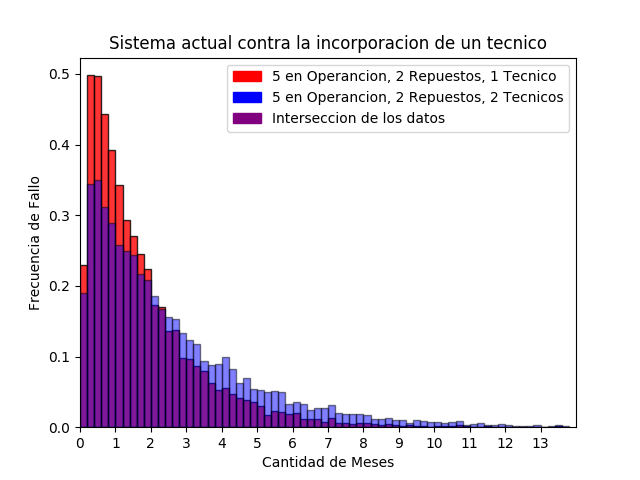
\includegraphics{Figure_1}

Mientras que la configuraci\'on actual tiene una tendencia a centrar los datos entre 0 y 1 mes, teniendo los picos m\'as altos (i.e. la mayor concentraci\'on de resultados) antes del primer mes. La contrataci\'on de un nuevo t\'ecnico hace que esta concentraci\'on se vea extendida hasta cerca de los 2 meses.
Al quedar la gr\'afica azul por encima de la roja por m\'as tiempo implica que la media obtenida, como se puede ver en la tabla, aument\'o casi un mes por sobre el sistema original. \\

\smallbreak
\subsubsection{Incorporaci\'on de una nueva lavadora}
En el siguiente gr\'afico se comparan los resultados obtenidos del tiempo medio de falla del sistema actual, contra la compra de una nueva lavadora. 

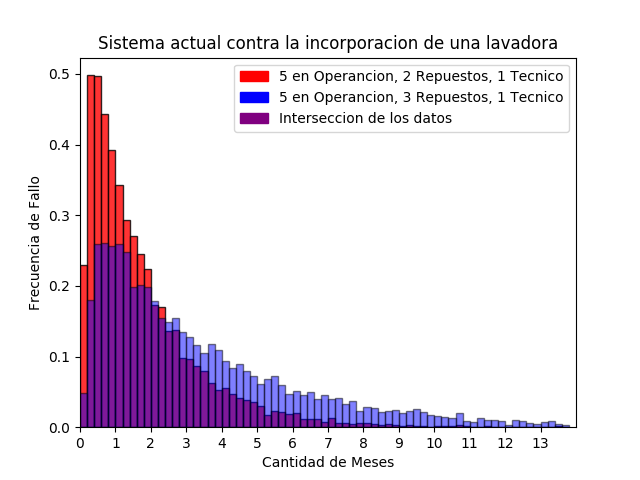
\includegraphics{Figure_2}

En este gr\'afico vemos que la incorporaci\'on de una nueva lavadora mejora a\'un m\'as el tiempo medio de vida, ya que en casi toda la extensi\'on del histograma la gr\'afica azul queda por encima de la roja.


\smallbreak
\subsubsection{Comparaci\'on de las dos opciones}

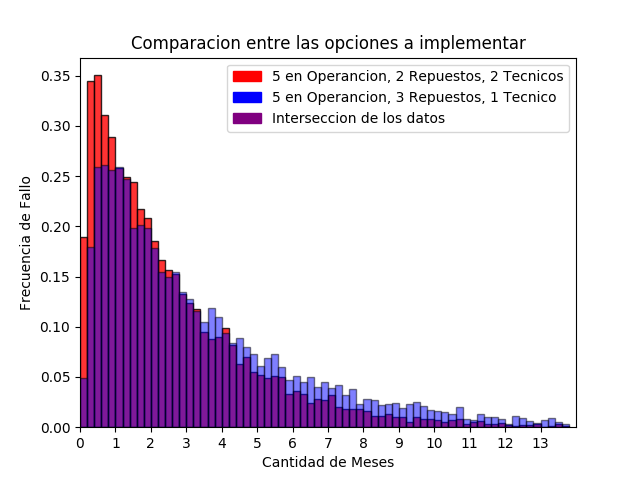
\includegraphics{Figure_3}
En las gr\'aficas previas notamos que ambas opciones mejoraban el sistema actual, en esta gr\'afica podemos ver, tal como lo muestran los datos tabulados. Que la opci\'on de adquirir una nueva lavadora es la que aumenta el tiempo medio de vida del sistema en mayor medida.

\section{Conclusiones}
A partir de los datos obtenidos en las simulaciones, se puede concluir, que la opci\'on de contratar un nuevo t\'ecnico aumentar\'a el tiempo de vida del lavadero en alrededor de un mes, mientras que adquirir una nueva lavadora manteniendo un s\'olo t\'ecnico contratado es la opci\'on que aumentar\'a de modo m\'as significativo el tiempo de vida del servicio, llevandol\'o a un tiempo esperado de vida de 3.66 Meses. Dado que ambas opciones aumentan el tiempo medio de vida del sistema, queda a consideraci\'on del dueño del Lavadero que opci\'on escoger en base a los costos que generan estas dos nuevas opciones. Nuestra recomendaci\'on en base a los datos observados es la compra de una nueva m\'aquina lavadora.

\section{Referencias}

\label{repositorio}
[1]\href{https://github.com/mrcmoresi/MyS17/}{C\'odigo fuente de la simulaci\'on}

\label{libro}
[2] Simulation. Sheldon M Ross. Quinta Edici\'on.



\end{document}
